% !TeX spellcheck=en_GB
%\documentclass{beamer}
\documentclass[handout]{beamer}
\usepackage{etex}
%% % use this with the [handout] option to create handouts for the audience
% \usepackage{pgfpages}
% \pgfpagesuselayout{2 on 1}[a4paper,border shrink=5mm]

\mode<presentation>
{
  \usetheme{Diku}
  % set this to your preferences:
  \setbeamercovered{invisible}
  %\setbeamercovered{transparent}
}
\usepackage{listings}
\usepackage{framed}
\usepackage{graphicx}
\usepackage{adjustbox}
\usepackage{epic}
\usepackage{url}
\usepackage{paratype}
\usepackage{xcolor}
\usepackage{ulem}
\usepackage{multirow}
\usepackage[utf8]{inputenc}
\usepackage{caption}
\usepackage{mathrsfs}
\setbeamerfont{frametitle}{family=\bf}


\setbeamertemplate{bibliography item}{\insertbiblabel}

\usepackage{amsmath}
\usepackage{amssymb}
\usepackage{amsthm}

\newcommand{\basetop}[1]{\vtop{\vskip-1ex\hbox{#1}}}
\newcommand{\source}[1]{\let\thefootnote\relax\footnotetext{\scriptsize\textcolor{kugray1}{Source: #1}}}
\definecolor{mygreen}{RGB}{50, 96, 60}

\lstdefinelanguage{Futhark}
{keywords={fun,if,then,else,loop,do,map,reduce,filter,scan,redomap,transpose,reshape,iota,replicate,let,in,for,while,with,f32,int,zip,streamRed,zipWith, unsafe, done, return},% done,return is a hack <- pseudocode not futhark
  sensitive=true,%
  comment=[l]{--},%
  string=[b]",%
  moredelim=**[is][\color{red}]{@}{@},
  moredelim=**[is][\color{blue}]{¤}{¤},
}

\lstset{
  language=Futhark,
  basicstyle=\footnotesize
}

% for coloured code citation in text:
\usepackage{fancyvrb}

%%%%%%%%%%%%%%%%%%%%%%%%%%%%%%%%%
%%%%% code sections   %%%%%%%%
%%%%%%%%%%%%%%%%%%%%%%%%%%%%%%%%%

% code highlighting commands in own block
\DefineVerbatimEnvironment{code}{BVerbatim}{}
\DefineVerbatimEnvironment{icode}{Verbatim}{fontsize=\scriptsize}
\DefineVerbatimEnvironment{tinycode}{Verbatim}{fontsize=\tiny}

% Fancy code with color commands:
\DefineVerbatimEnvironment{colorcode}%
{Verbatim}{fontsize=\scriptsize,commandchars=\\\{\}}
\DefineVerbatimEnvironment{smallcode}%
{Verbatim}{fontsize=\tiny,commandchars=\\\{\}}

%%%%%%%%%%%%%%%%%%%%%%%%%%%%%%%%%%
%%%%% some coloring    %%%%%%%%

% use "DIKU green" from our color theme for \emph
\renewcommand{\emph}[1]{\textcolor{structure}{#1}}
% use some not-too-bright red for an \emp command
\definecolor{DikuRed}{RGB}{130,50,32}
\newcommand{\emp}[1]{\textcolor{DikuRed}{ #1}}
\definecolor{CosGreen}{RGB}{10,100,70}
\newcommand{\emphh}[1]{\textcolor{CosGreen}{ #1}}
\definecolor{CosBlue}{RGB}{55,111,122}
\newcommand{\emphb}[1]{\textcolor{CosBlue}{ #1}}
\definecolor{CosRed}{RGB}{253,1,1}
\newcommand{\empr}[1]{\textcolor{CosRed}{ #1}}

\newcommand{\mymath}[1]{$ #1 $}
\newcommand{\myindx}[1]{_{#1}}
\newcommand{\myindu}[1]{^{#1}}

\newcommand{\myalt}{~|~}

\makeatletter
\long\def\beamer@author[#1]#2{%
  \def\insertauthor{\def\inst{\beamer@insttitle}\def\and{\beamer@andtitle}%
    \begin{tabular}{lr}#2\end{tabular}}%
  \def\beamer@shortauthor{#1}%
  \ifbeamer@autopdfinfo%
  \def\beamer@andstripped{}%
  \beamer@stripands#1 \and\relax
  {\let\inst=\@gobble\let\thanks=\@gobble\def\and{, }\hypersetup{pdfauthor={\beamer@andstripped}}}
  \fi%
}
\makeatother

%%%%%%%%%%%%%%%%%%%%

\title{Programming Massively Parallel Hardware\\\textbf{Simplex on the GPU}}

\author[]{%
  Anders Wind Steffensen \\
  Chi Pham \\
  Michael Hejselbak Jensen \\
}

\institute{Department of Computer Science (DIKU)\\University of Copenhagen}


\date[3/3]{November 9th 2017}


\begin{document}

\titleslide

%%%%%%%%%%%%%%%%%%%%%%%%%%%%%%%%%%%%%%%%%%%%%%%%%%%%%%%%%%%%%%%%%%%%%%

\begin{frame}
  \frametitle{Overview}
  \begin{itemize}
  \item Introduction
  \item Design
  \item Implementation
  \item Design
  \item Results
  \item Conclusion
  \end{itemize}
\end{frame}

%%%%%%%%%%%%%%
% INTRO
%%%%%%%%%%%%%%

\begin{frame}[fragile]
\frametitle{Futhark test}
Futhark test
\pause
\begin{lstlisting}
// @emphasis@
// ¤emphasis2¤
let simplex [n] [m] (A : [m][n]f32) (b : [m]f32)
  (c : [n]f32) (v : f32) =
  let e = entering_variable c
  let (_,_,_,v,_) = loop (A,b,c,v,e) while e != -1 do
    let l = leaving_variable A b e
    let (A,b,c,v) = unsafe pivot A b c v l e
    let e = entering_variable c
    in (A,b,c,v,e)
  in v

\end{lstlisting}
\end{frame}

%%%%%%%%%%%%%%
% DESIGN
%%%%%%%%%%%%%%
\begin{frame}
\frametitle{Motivation}
\begin{itemize}
	\item Linear programming is widely used technique for optimization.
	\item Simplex is the most used algorithm to solve Linear programs.
	\item To our knowledge there has not been done work on parallelism across multiple instances on massively parallel hardware.
\end{itemize}
\end{frame}

\begin{frame}
\frametitle{Focus}
\begin{itemize}
	\item Implement fast parallel versions of Simplex.
	\item Experiment with parallelism across multiple instances of Simplex.
	\item Benchmark different solutions and compare with 'state of the art' implementation.
\end{itemize}
\end{frame}


\begin{frame}
\frametitle{Simplex}
\begin{itemize}
	\item Pivots variables to increasingly increase the objective value.
	\item After each pivot new constraint matrix, coefficients and constants form the next basis.
	\item The number of pivots is in worst case exponential and is required to run sequentially.
\end{itemize}
\end{frame}

\begin{frame}[fragile]
\frametitle{Multi-Simplex}
\begin{lstlisting}
Multi-Simplex(As[h][m][n], bs[h][m], cs[h][n]) =
  map
    (\A b c ->
      v = 0
      e = Entering-Variable(c)
      while (e != -1) do
        @l = Leaving-Variable(A,b,e)
        (A,b,c,v) = Pivot(A,b,c,v,e,l)
        e = Entering-Variable(c)@
      done
      return v
    )
    As bs cs

Entering-Variable(c[n]) = @reduce, iota@
Leaving-Variable(A[m][n], b[m], e) = @map, reduce, iota@
Pivot(A[m][n], b[m], c[n], v, e, l) = @map, iota@
\end{lstlisting}
\end{frame}

\begin{frame}
\frametitle{Design}
\begin{itemize}
	\item \textbf{Outer parallel}: Instances are computed in parallel. Simplex is not parallelized. Flattening is not needed.
	
	\item \textbf{Inner parallel}: Simplex is computed in parallel. Not parallel across instances. Small degree of flattening.
	
	\item \textbf{Fully parallel}: Simplex and instances are computed in parallel. High degree of flattening.
\end{itemize}
\end{frame}

\begin{frame}
\frametitle{Design}
Observations:
\begin{itemize}
	\item In the fully parallel version, the overhead of flattening is amortized over the number of pivots.
	
	\item Each pivot is mostly map operators, minimizing synchronization.
	
	\item other positive things?
\end{itemize}
\end{frame}

\begin{frame}
\frametitle{Design}
Observations:
\begin{itemize}
	\item The convergence loop is the hard limit on parallisation. Worst case exponential. 
	
	\item Busy work when number of pivots differ across instances.
	
	\item other negative things?
\end{itemize}
\end{frame}

%%%%%%%%%%%%%%
% IMPLEMENTATION
%%%%%%%%%%%%%%

\begin{frame}
	\frametitle{Test generation}
	\begin{itemize}
		\item Parametrized on \#instances, \#variables, \#constraints, range of random values
		
		\item Each parameter affects the running time significantly. The significance of values is not immediately obvious.
		
		\item Superfluous constraints and variables.
	\end{itemize}
\end{frame}

\begin{frame}
\frametitle{Benchmark categories}
\begin{itemize}
	\item \textbf{One Big Instance}: Stresses the implementations ability to compute Simplex.
	
	\item \textbf{Many Small Instances}: Stresses the implementations ability to compute Simplex many times where each computation of simplex is diminished.
	
	\item \textbf{Many Big Instances}: Stresses the implementations ability to compute simplex many times where each iteration of Simplex is significant. 
	
	\item \textbf{Many Varying Instances}: Stresses the implementations ability to compute simplex over many instances where simplex might or might not be significant. 
\end{itemize}
\end{frame}

%%%%%%%%%%%%%%
% RESULTS
%%%%%%%%%%%%%%
\begin{frame}[fragile]
\frametitle{One Big Instance}
\centering
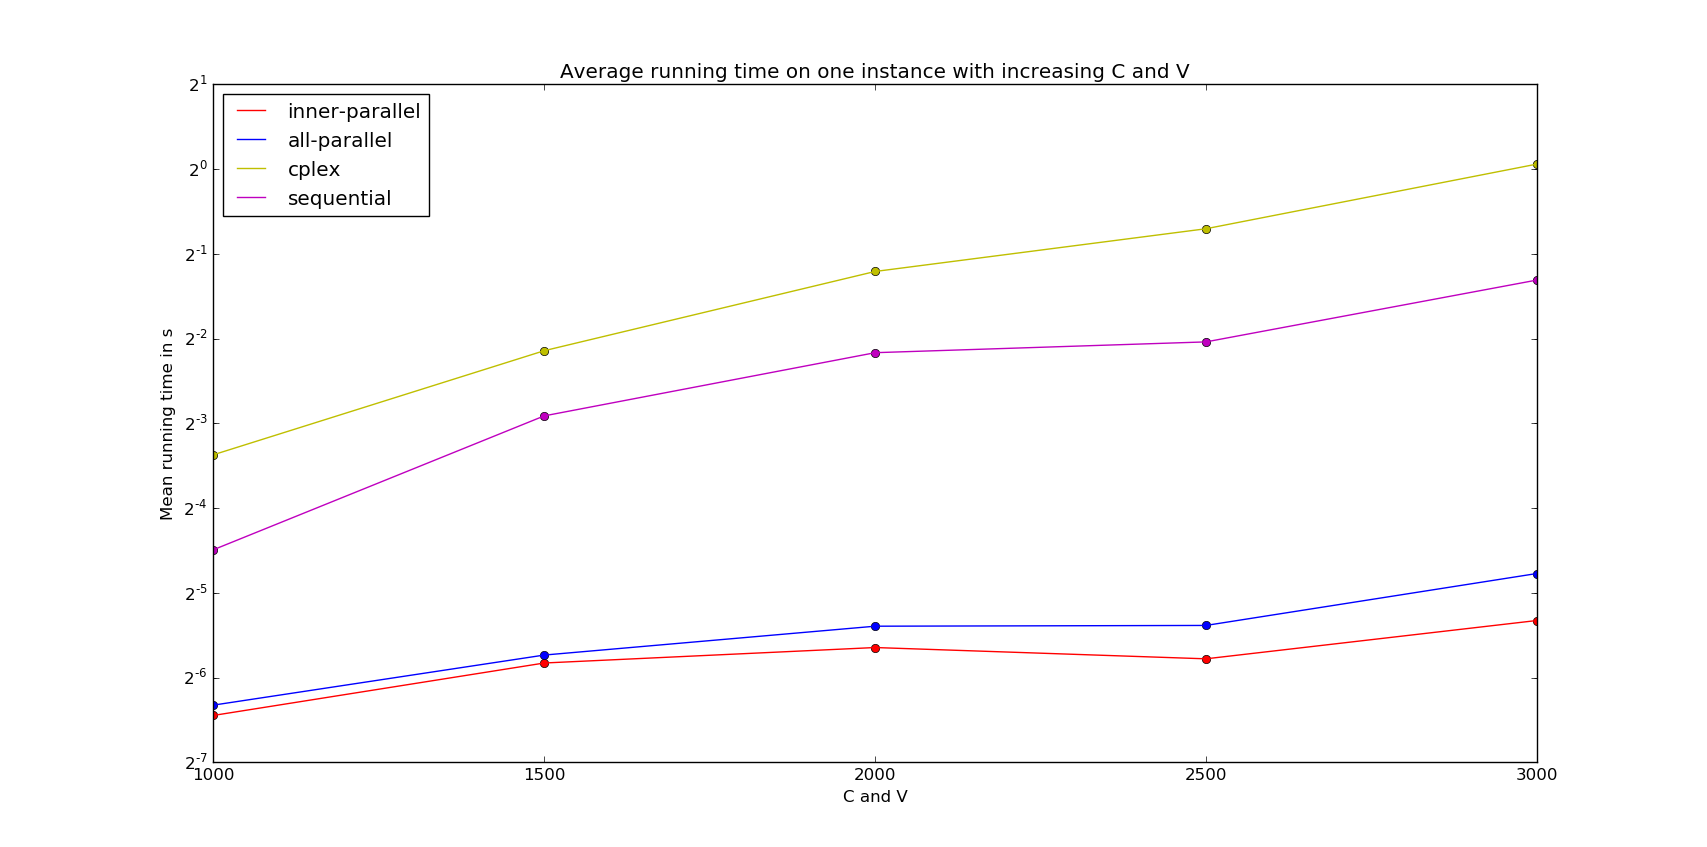
\includegraphics[width=0.9\textwidth]{../Doc/figures/one-big}
\begin{itemize}
	\item Inner parallel ~15??? times faster than Futhark-c
	\item Fully parallel is slightly slower than inner. 
	\item CPLEX algorithmic optimizations
\end{itemize}
\end{frame}

\begin{frame}[fragile]
\frametitle{Many Small Instance}
\centering
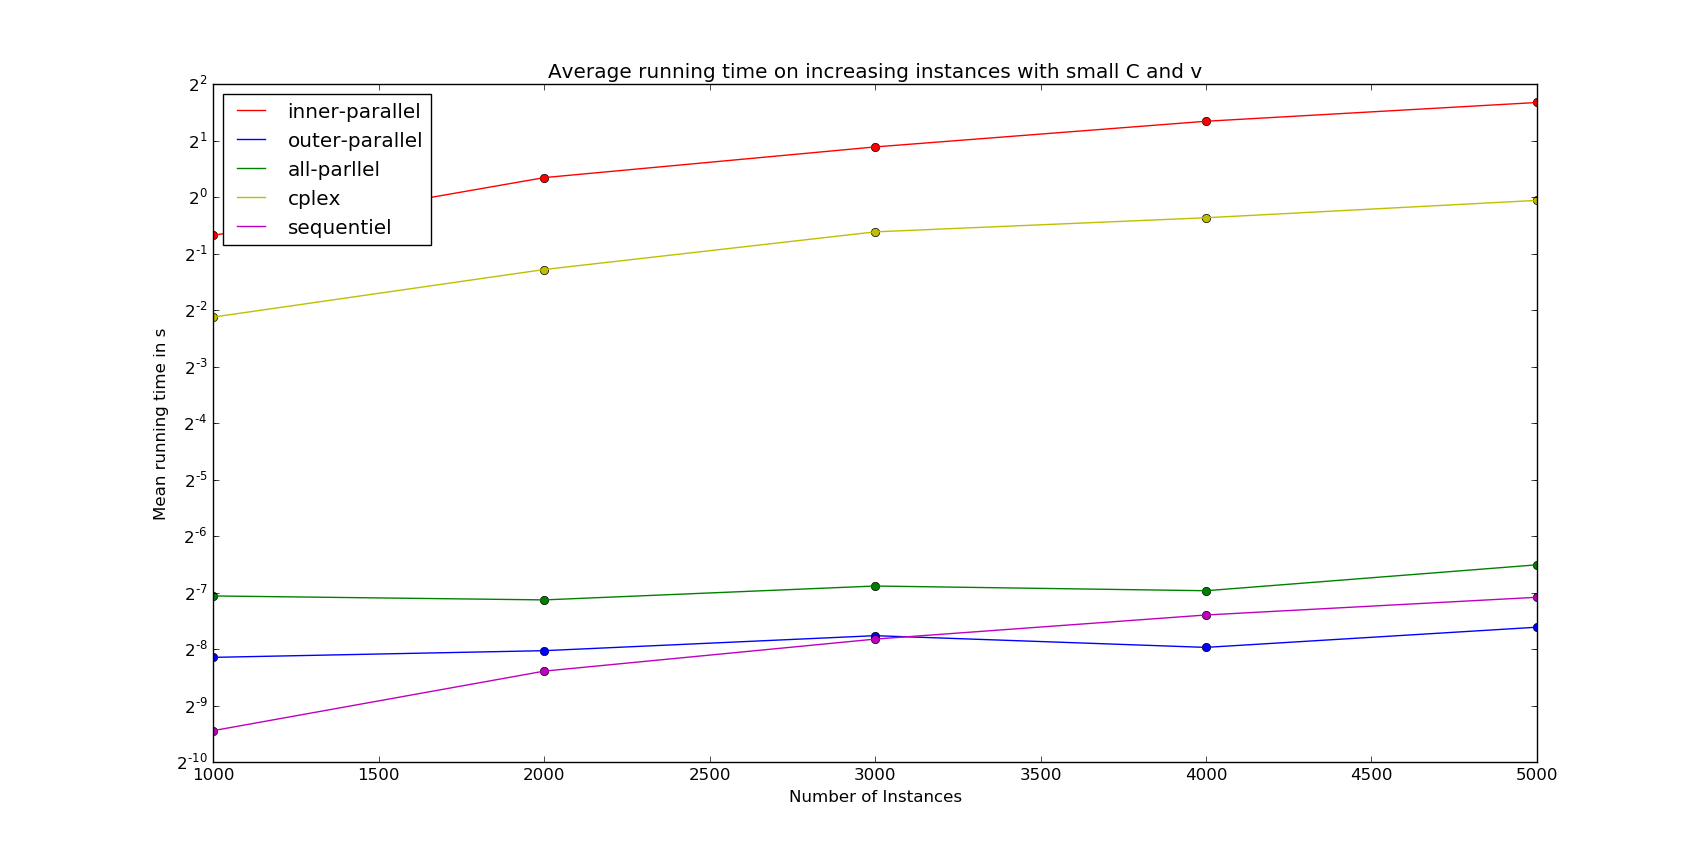
\includegraphics[width=0.85\textwidth]{../Doc/figures/many-small}
\begin{itemize}
	\item Outer parallel only faster than Futhark-c for high number of instances.
	\item Fully parallel is slightly slower than outer and sequential. 
	\item Calculation of simplex is more important than parallelization across instances.
	\item CPLEX not optimized for solving multiple. Maybe overhead in preprocessing.
\end{itemize}
\end{frame}

\begin{frame}[fragile]
\frametitle{Many Big Instance}
\centering
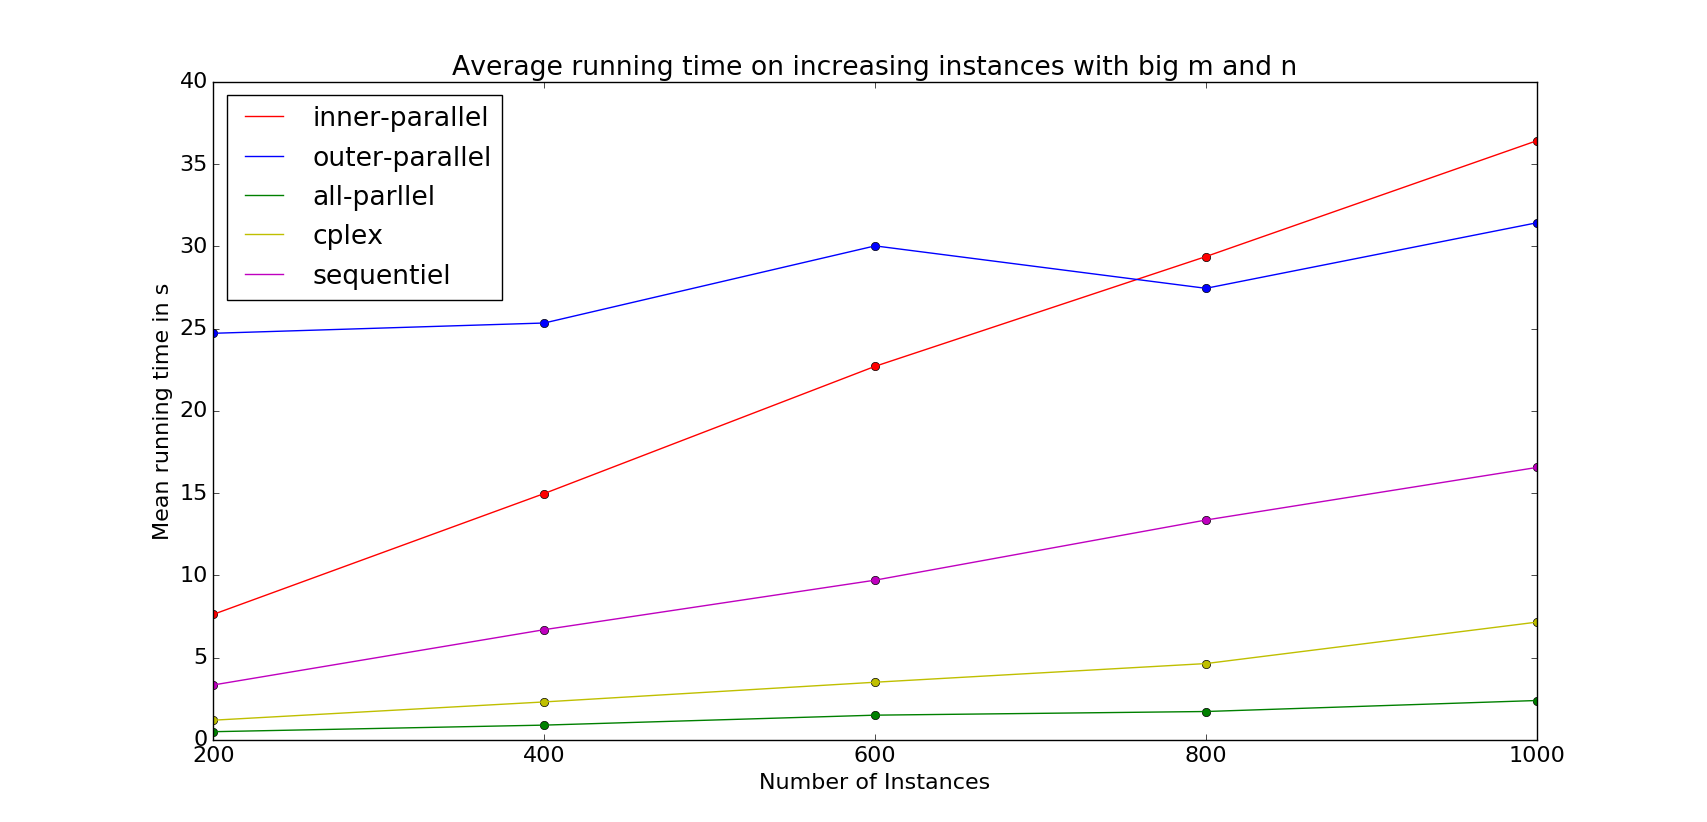
\includegraphics[width=0.9\textwidth]{../Doc/figures/many-big}
\begin{itemize}
	\item Fully parallel x times faster than sequential and x times faster than CPLEX.
	\item Sequential code is faster than either parallization on inner or outer only.
\end{itemize}
\end{frame}

\begin{frame}[fragile]
\frametitle{Many Instance of Varying Size}
\centering
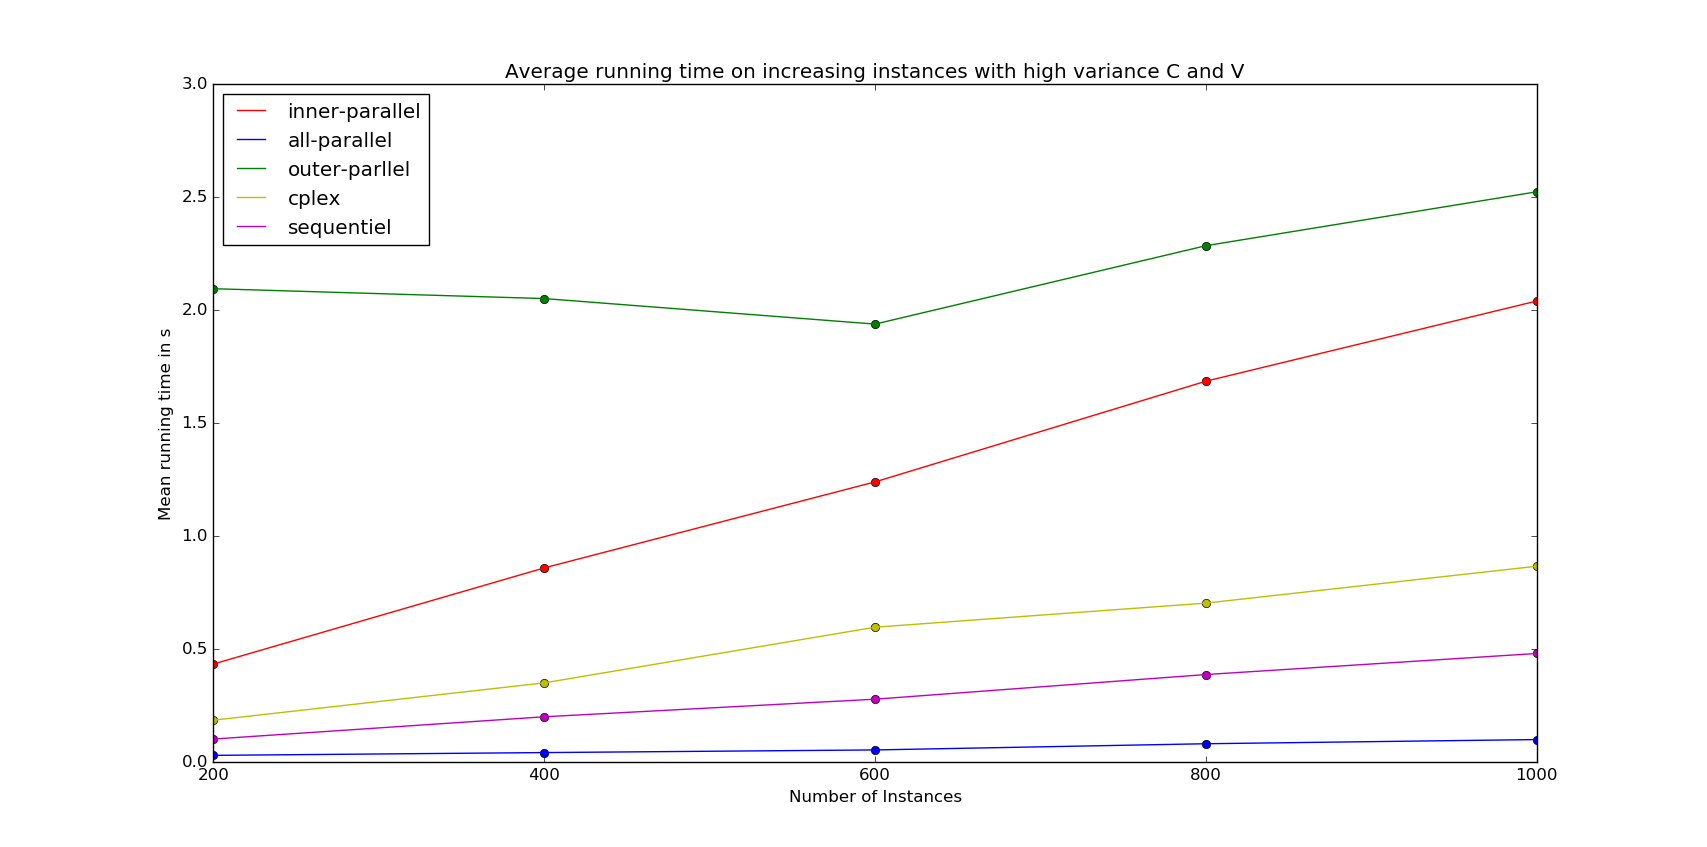
\includegraphics[width=0.9\textwidth]{../Doc/figures/many-varying}
\begin{itemize}
	\item Fully parallel x times faster than sequential and x times faster than CPLEX.
	\item Fully parallel ambivalent on sizes.
\end{itemize}
\end{frame}

\begin{frame}
\frametitle{Evaluation (needs some work)}
\begin{itemize}
\item Outer and fully parallel versions do well for multiple instances
\item Inner parallel is not much better than fully parallel
\item For bigger instances, CPLEX seems to scale way better
\item Something with numbers and x speedup
\end{itemize}
\end{frame}

\begin{frame}
\frametitle{Improving the Results}

If the convergence loop is our bottleneck, what can we do?

\begin{itemize}
\item Decrease the overhead of an iteration
\item Decrease the number of iterations ($\leftarrow$ CPLEX!!!)
\end{itemize}

\begin{figure}
\begin{tabular}{|c|c|c|c|c|}
\hline
\textbf{Number of instances} & \textbf{Size range} & \textbf{Mean} & \textbf{Standard deviation} \\\hline
5000 & 1-10 & 3.772 & 2.630 \\\hline
3000 & 10-150 & 77.192 & 53.616 \\\hline
1000 & 150-200 & 254.283 & 79.926 \\\hline
1 & 5000 & 57994 & 0 \\\hline
\end{tabular}
\caption{Mean number of iterations}
\end{figure}
\end{frame}

\begin{frame}
\frametitle{Improving the Results}
An experiment: unrolling some of the loop iterations

Loop unrolling: Futhark double buffer memcpy loop

TODO: graph for loop unrolled results
\end{frame}

%%%%%%%%%%%%%%
% CONCLUSION
%%%%%%%%%%%%%%

\begin{frame}
\frametitle{Further Work}
\begin{itemize}
	\item Experiment to clarify for what sizes and what number of instances the fully parallel does better than CPLEX.
	\item Preprocessing to decrease size and number of iterations
	\item Better rules for finding entering and leaving variable. Compute multiple pivots from same basis in parallel and pick best.
\end{itemize}
\end{frame}
\end{document}
